\chapter{Hypergeometric-type Series Containing Digamma Function}
\label{ch_4}

This chapter will focus on the properties and behavior of the hypergeometric-type series containing a digamma function as a factor. From the previous chapter, we see how this type of series naturally appears in the calculation of the finite-part integration. There are already few papers that got interested in this type of series. The series was first tabulated in \cite{hansen1975table} but still there remains a significant gap. The exploitation of this series to produce a reduction formula of the Kampé de Fériet function can be seen in \cite{miller2006summations} and \cite{cvijovic2008closed}.

The chapter will start on the definition of hypergeometric-type series containing a digamma function as a factor. Next, we will establish its convergence and singularity. Then, if not defined on the whole complex plane, we will implement the concept of analytic continuation to extend the region of its analyticity. The goal is to find a representation of the series that will cover the whole complex plane and broaden the restrictions of each parameter. Lastly, we will derive the relation of this generalized series to the Kampé de Fériet function.

\section{Definitions}
The series 
\begin{align}
\begin{split}
      \psi(c) & + \frac{a_1 a_2 \dots a_p}{b_1 b_2 \dots b_q} \psi(c+1) \frac{z}{1!} \\& + \frac{a_1(a_1+1) a_2(a_2+1) \dots  a_p(a_p+1)}{b_1(b_1+1) b_2 (b_2+1) \dots b_q(b_q+1)} \psi(c+2) \frac{z^{2}}{2!} + \dots \\& \hspace{40mm} = \sum_{k=0}^{\infty} \frac{\prod_{l=1}^{p} (a_{l})_k}{ \prod_{l=1}^{q} (b_{l})_k} \psi(k+c) \frac{z^k}{k!}.
\end{split}
\end{align}
is a hypergeometric-type series containing a digamma function as a factor. It has a parameter of $\Vec{a}$, $\Vec{b}$, $c$, and $z$. Take note that $\Vec{a}$ means $a_1, a_2, \dots, a_p$ and $\Vec{b}$ corresponds to $b_1, b_2, \dots, b_q$. Any of these quantities may be real or complex. However, the parameter $\Vec{b}$ and $c$ must not be negative integers since they will make the series undefined. In addition, if any of the $a$ parameters is a negative integer, the function will reduce to a polynomial.  If the sum of the series exists, it will be denoted by the symbol 
\begin{equation}
    \pPq{p}{q}{\Vec{a}}{\Vec{b}}{c}{z}.
\end{equation}
Finally, we define the function $_{p}\tilde{\psi}_{q}$ with series representation of
\begin{equation} \label{psi}
    \pPq{p}{q}{\Vec{a}}{\Vec{b}}{c}{z} =  \sum_{k=0}^{\infty} \frac{\prod_{l=1}^{p} (a_{l})_k}{ \prod_{l=1}^{q} (b_{l})_k} \psi(k+c) \frac{z^k}{k!}.
\end{equation}
Obviously, the function $_{p}\tilde{\psi}_{q}$ is an analytic function since it is defined as a power series whenever the series converges.

\section{Convergence of the general series}

In studying an infinite series, the first thing we are interested in is its convergence. There are a lot of existing tests to tell if the series will diverge or converge. Most of the known tests can be found in \cite{hardy2018course}.

In general, a complex power series $\sum^{\infty} a_k z^k$ is said to converge only for certain values of $z$. This region is an open disk with radius $R$, where the number $R$ is called the radius of convergence. The power series will always converge absolutely for all the values of $z$ inside the open disk and will diverge outside it. On the boundary of the disk, the behavior of the power series is said to be complicated since it may converge or diverge \cite{hardy1940ramaniyan}. Therefore, it is important to determine the number $R$ or the radius of convergence to establish the convergence of the series. There are many ways to determine the radius of convergence $R$ of the series. In this discussion, we will use the so-called ratio test or d'Alembert's test to determine the radius of convergence of the function ${}_{p}\tilde{\psi}_q$. The test requires as to find the limits of the ratio of two successive terms $u_k$ and $u_{k+1}$ of the series so that as $k \to \infty$, the ratio 
\begin{equation}
    \left| \frac{u_{k+1}}{u_k} \right| \to \left| z \right|.
\end{equation}
According to the test, the series is convergent for all values of $z$, real or complex such that $|z| < 1$, and it will diverge for all the values of $z$ real or complex, such that $|z| > 1$. A more delicate test needed for the boundary $|z| = 1$. 

Implementing the convergence test, we will define $L$ as
\begin{equation} \label{RT}
    L = \lim_{k \to \infty} \left| \frac{u_{k+1}}{u_k} \right| 
\end{equation}
and we identified the $k$th term as
\begin{equation}
    u_k = \frac{\prod_{l=1}^{p} (a_{l})_k}{ \prod_{l=1}^{q} (b_{l})_k} \psi(k+c) \frac{z^k}{k!}.
\end{equation}
Identifying the two successive terms using the above equation and substituting it to equation \eqref{RT} will result to
\begin{equation} \label{RTA}
    L = \lim_{k \to \infty} \left| \frac{\frac{ \prod_{l=1}^{p} (a_{l})_{k+1}}{ \prod_{l=1}^{q} (b_{l})_{k+1}} \psi(k+1+c) \frac{z^{k+1}}{(k+1)!}}{\frac{ \prod_{l=1}^{p} (a_{l})_k}{ \prod_{l=1}^{q} (b_{l})_k} \psi(k+c) \frac{z^k}{k!}} \right|.
\end{equation}
Using the fact that
\begin{equation}
    \frac{ \prod_{l=1}^{p} (a_{l})_{k+1}}{ \prod_{l=1}^{p} (a_{l})_{k}} = \prod_{l=1}^{p} (k+a_l).
\end{equation}
and 
\begin{equation}
    \frac{\psi(k+c+1)}{\psi(k+c)} = 1 + \frac{1}{(k+c)\psi(k+c)}
\end{equation}
equation \eqref{RTA} will reduce to 
\begin{align}
\begin{split} \label{RTA2}
    L &= \lim_{k \to \infty} \frac{|k+a_1||k+a_2| \dots |k+a_{p}|}{|k+b_1||k+b_2| \dots |k+b_{q}|} \left| 1 + \frac{1}{(k+c)\psi(k+c)} \right| \frac{|z|}{|k+1|} 
    \\& = \lim_{k \to \infty} |z| \, k^{p-q-1}  \frac{ (1+|a_1|/k)(1+|a_2|/k) \dots (1+|a_{p}|/k)}{(1+1/k) (1+|b_1|/k)(1+|b_2|/k) \dots (1+|b_{q}|/k)} \\& \hspace{65mm} \times \left( 1 + \frac{1}{|(k+c)\psi(k+c)|} \right).
\end{split}
\end{align}
From the result, we can conclude that the value $L$ or the limits will purely depend on the value of $p$ and $q$. It is trivial to see that when $p \leq q $, the series $_{p}\tilde{\psi}_{q}$ converges for all values of $z$, real or complex since the value of $L$ tends to zero as $k \to \infty$. 

Also, when $p > q + 1 $ the value of $L$ will tend to infinity. It implies that the series will never converge unless $z=0$, and under this condition, the function is only defined when the series terminates, that is when one or more of the $a$ parameters is zero or a negative integer. Lastly, for the case where $p = q+1$, the value of $L$ will tend to $|z|$. This means that the convergence of the series is dependent on the value of $z$. The series is convergent for $|z| < 1$ and will diverge for $|z| > 1$. A more delicate test is needed to investigate the behavior of the series at $|z| = 1$.

When $|z| = 1$ and $p = q+1$, equation \eqref{RTA} can be approximated as
\begin{align}
\begin{split}
    L &= \lim_{k \to \infty} \left(1 + \frac{\sum_{l=1}^{p} \mathrm{Re}(a_l)}{k} + \mathcal{O}\left( \frac{1}{k^2}\right)\right) \left(1 - \frac{\sum_{l=1}^{q} \mathrm{Re}(b_l)}{k} + \mathcal{O}\left( \frac{1}{k^2}\right)\right)
    \\& = \lim_{k \to \infty} \left(1 + \frac{\sum_{l=1}^{p} \mathrm{Re}(a_l) - \sum_{l=1}^{q} \mathrm{Re}(b_l)-1} {k} + \mathcal{O}\left( \frac{1}{k^2}\right)\right).
\end{split}
\end{align}
By Raabe's test \cite{10.2307/24338342}, for $z=1$, the series will converge if
\begin{equation}
    \mathrm{Re}\left(\sum_{l=1}^{q} b_l- \sum_{l=1}^{p} a_l \right) > 0,
\end{equation}
and when $z=-1$, it will converge for 
\begin{equation}
    \mathrm{Re}\left(\sum_{l=1}^{q} b_l- \sum_{l=1}^{p} a_l \right) > -1.
\end{equation}
For the other point in the boundary, the case where $|z| = 1$, but $z \neq 1$. the series is absolutely convergent if 
\begin{equation} \label{converge}
    \mathrm{Re}\left(\sum_{l=1}^{q} b_l- \sum_{l=1}^{p} a_l \right) > 0,
\end{equation}
and conditionally convergent for
\begin{equation}
    -1 < \mathrm{Re}\left(\sum_{l=1}^{q} b_l- \sum_{l=1}^{p} a_l \right) \leq 0.
\end{equation}

We see that the series is analytic only at the region of $|z| < 1$ when $p = q +1$, this region is called the circle of convergence of the function. The next goal now is to extend its analyticity outside the circle of convergence. Before this, we need to show that the boundary is not a natural boundary since it will determine if the analytic continuation is possible. 

In general, the boundary of the circle of convergence of a power series has at least one singular point. If a boundary is a natural boundary, any point on it is a singularity. To show the nature of the boundary, one will immediately implement the standard method of analytic continuation, the series expansion. Luckily, we can know its nature right away by using Fabry's gap Theorem \cite{2008189}, we can easily show that the boundary of $_{q+1}\tilde{\psi}_{q}$ is not a natural boundary. According to Fabry's gap theorem, suppose $f(z)=\sum u_k z^{k_n}$ and has a radius of convergence $R$, if the limit 
\begin{equation}
    M = \lim_{k \to \infty} \frac{k_n}{k},
\end{equation}
approaches infinity, then the boundary is a natural boundary. Applying the theorem to the function $_{q+1}\tilde{\psi}_{q}$, we found that the value of M is equal to 1. By the converse of the theorem, we can say that the boundary of the circle of convergence of function $_{q+1}\tilde{\psi}_{q}$ is not a natural boundary. Thus, it is possible to extend the analyticity of the function $_{q+1}\tilde{\psi}_{q}$ to the whole complex plane. 

Additionally, by Fabry's quotient theorem \cite{fabry1896points}, we can easily show locate the singular point of the function $_{q+1}\tilde{\psi}_{q}$. According to this theorem, if the coefficients of the power series with unit radius of convergence, satisfy the condition 
\begin{equation}
    \lim_{k \to \infty} \frac{u_{k+1}}{u_k}  = s,
\end{equation}
then $z=s$ is a singular point of the function. Applying the theorem on the function $_{q+1}\tilde{\psi}_{q}$, by equation \eqref{RTA}, we can easily found that the singular point is located at $z=1$.

\section{Singularities of the function ${}_{p}\tilde{\psi}_{q}$}

Before we extend the analyticity of the function, we will first discuss the singularities of the function ${}_{p}\tilde{\psi}_{q}$ and its nature.

\subsection{Poles and essential singularity}

For the non-polynomial case, we can only have an essential singularity at infinity when $p \leq q$. 

For the polynomial case, that is when at least one of the $a$ parameter is negative, at any value of $p$ and $q$ the series will have a pole singularity with a pole of order $min(-a_1, -a_2, \dots, -a_p )$ at the infinity. 

If we analyze the function with respect to its parameters $a$, $b$, and $c$. All of the parameters will have an essential singularity at infinity. However, only parameters $b$ and $c$ will have simple poles at $\mathbb{Z}_{0}^{-}$. Those simple poles are acquired from the definition of gamma and digamma function.

\subsection{Branch point and branch cut}

The function ${}_{p}\tilde{\psi}_{q}$ can only have a branch point at $z = 1$ and at infinity for the case $p = q+1$. Lastly, we choose the branch cut to run along the positive real axis $[1, \infty]$.

\section{Analytic continuation of $_{q+1}\tilde{\psi}_{q}$}

Recall in the previous section, for $p = q + 1$, the function is not analytic on the whole complex plane. In this section, the goal is to extend the analyticity of the function $_{q+1}\tilde{\psi}_{q}$  to the whole complex plane using the concept of analytic continuation.  


\subsection{The standard method of analytic continuation}

The standard method of analytic continuation is the method of power series.  It is just performing a Taylor series expansion at the analytic region of the function. To fully understand this, we will use this method to extend the analyticity of our function ${}_{p}\tilde{\psi}_{q}$. Recall that the function ${}_{p}\tilde{\psi}_{q}$ is defined as a power series in equation \eqref{psi}. Also, this power series is said to converge only at $|z| < 1$ when $p = q+1$. Thus, the function is only analytic at the region $|z| < 1$. 

Next, we need to choose a point inside the region of convergence, let say, some arbitrary point $d$ that is $|d| < 1$. Performing a Taylor series expansion at that point will result to
\begin{equation}
    f(z) = \sum_{n=0}^{\infty} \left.\frac{\mathrm{d}}{\mathrm{d}z} \pPq{q+1}{q}{\vec{a}}{\vec{b}}{c}{z} \right|_{z=d} \frac{(z-d)^{n}}{n!}
\end{equation}

\begin{figure}
    \centering
    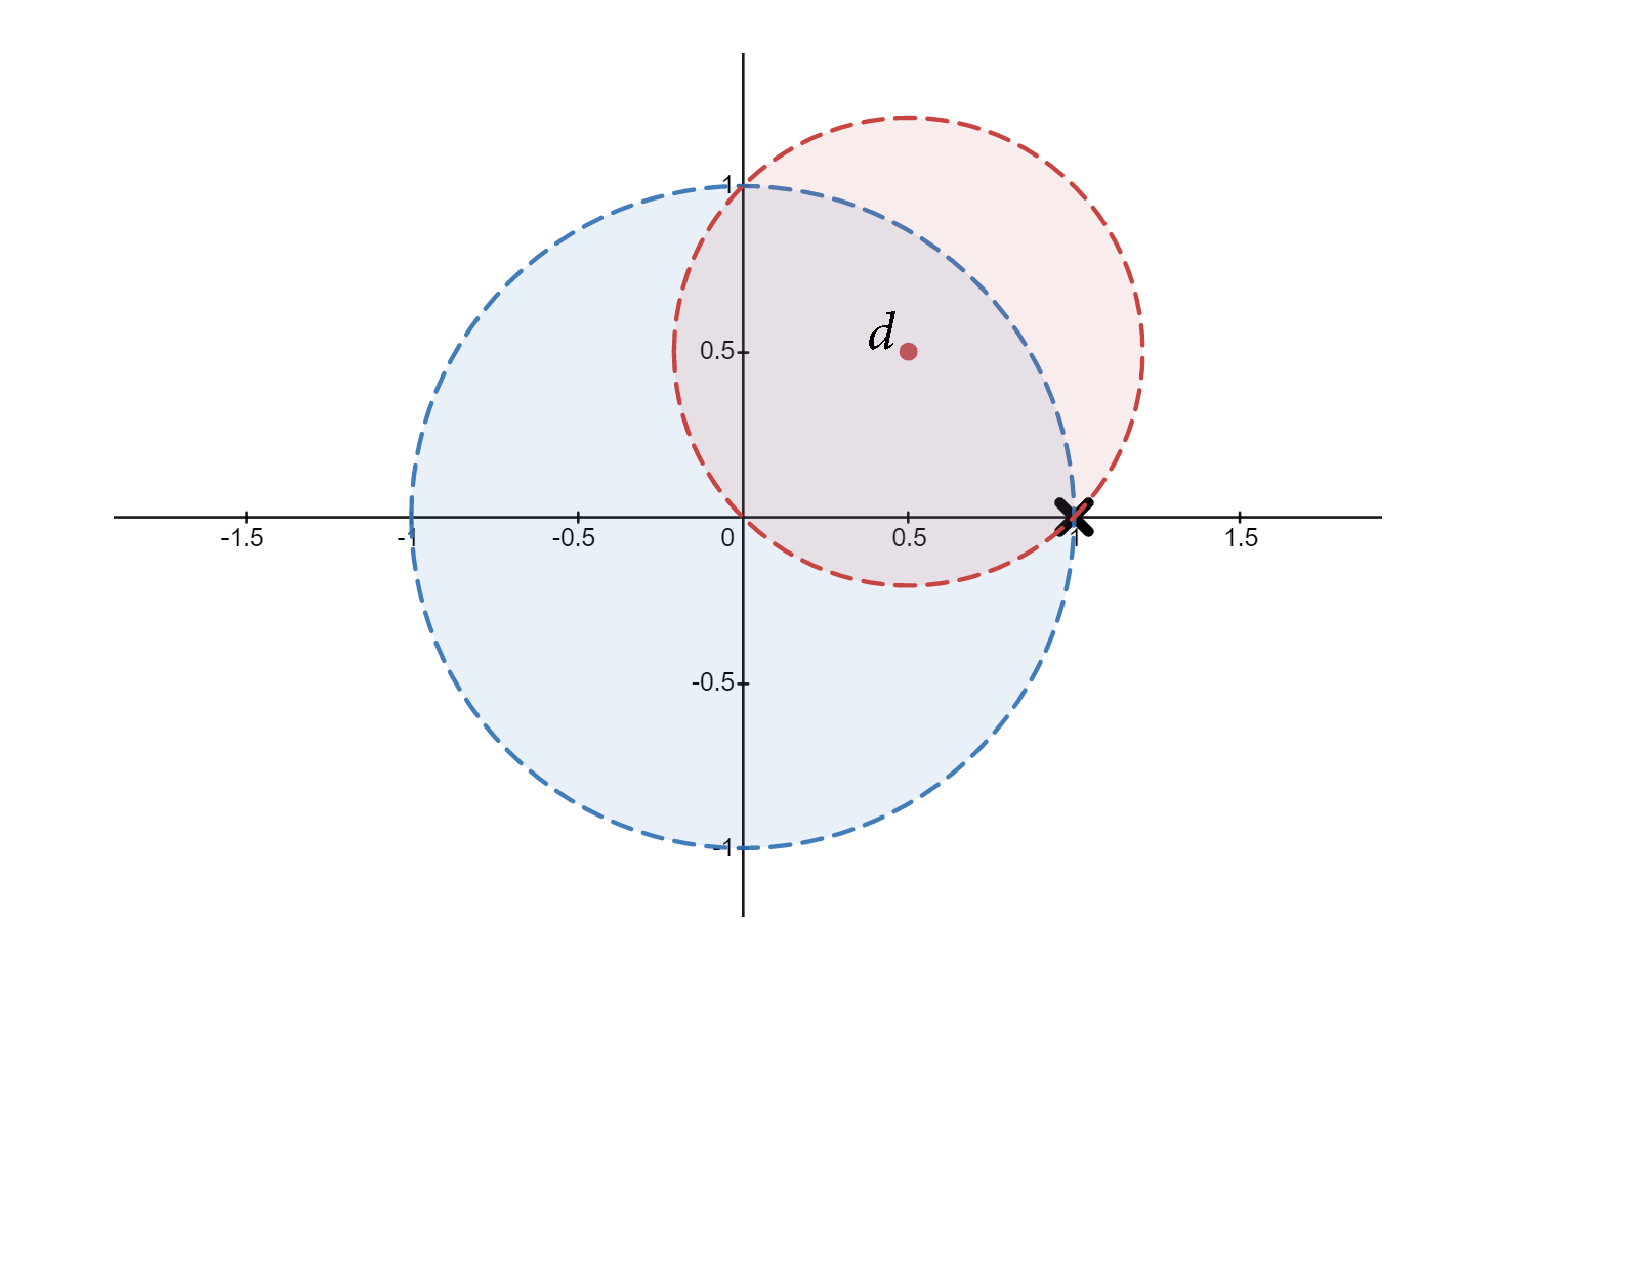
\includegraphics[width=.75\textwidth]{Taylor1.pdf}
    \caption{Graphical representation of the standard method of analytic continuation.}
    \label{Taylor1}
\end{figure}

The resulting series will absolutely converge in any circle centered at $d$ and that circle lies in the circle $|z| = 1$. This series may converge in a larger circle and will provide an analytic continuation of the function as shown in Figure \ref{Taylor1}.

Recall that our goal is to extend the analyticity to the whole complex plane. Thus, we need to perform infinitely many expansions to cover the complex plane. In this case, the standard method of analytic continuation is not practical to use. But, this is still useful if the goal is to extend the analyticity of the function to a specific region.

\subsection{Analytic continuation through the integral representation of digamma function}

We already showed that standard method of analytic continuation is not practical in extending the analyticity of the function to the whole complex plane. In that case, we need to think of a more clever way of extending the function analyticity. Using the zeta function as an inspiration, one may exploit the integral representation of the digamma function. 

One of the integral representation of the digamma function $\psi(z)$ \footnote{Digamma function has a simple pole for all negative integers including zero.} is 
\begin{equation} \label{DGIR}
    \psi(z) = \int_{0}^{1} \frac{1-t^{z-1}}{1-t} \, \mathrm{d}t - \gamma
\end{equation} 
where $\gamma$ is the Euler-Mascheroni constant and exists for $Re(z) > 0$. Directly substituting the above integral representation to the ${}_p\tilde{\psi}_{q}$ written in equation \eqref{psi}, we will have 
\begin{equation}
    \pPq{p}{q}{\Vec{a}}{\Vec{b}}{c}{z} =  \sum_{k=0}^{\infty} \frac{\prod_{l=1}^{p} (a_{l})_k}{ \prod_{l=1}^{q} (b_{l})_k} \left( \int_{0}^{1} \frac{1-t^{k+c-1}}{1-t} \, \mathrm{d}t - \gamma \right) \frac{z^k}{k!}.
\end{equation}
By invoking the convergence of the integral, we can now interchange the integral and summation, resulting to
\begin{align}
\begin{split} 
    \pPq{p}{q}{\Vec{a}}{\Vec{b}}{c}{z} & =\int_{0}^{1} \frac{\sum_{k=0}^{\infty} \frac{\prod_{l=1}^{p} (a_{l})_k}{ \prod_{l=1}^{q} (b_{l})_k} \frac{z^k}{k!} - \sum_{k=0}^{\infty} \frac{\prod_{l=1}^{p} (a_{l})_k}{ \prod_{l=1}^{q} (b_{l})_k} \frac{(tz)^k}{k!} t^{c-1}}{1-t} \, \mathrm{d}t \\& \qquad - \gamma \, \sum_{k=0}^{\infty} \frac{\prod_{l=1}^{p} (a_{l})_k}{ \prod_{l=1}^{q} (b_{l})_k} \frac{z^k}{k!}.
\end{split}
\end{align}
Rewriting the above equation by making the series into hypergeometric function written in equation \eqref{GHF} will result to
\begin{align}
\begin{split} 
    \pPq{p}{q}{\Vec{a}}{\Vec{b}}{c}{z} & =\int_{0}^{1} \frac{\pFq{p}{q}{\Vec{a}}{\Vec{b}}{z} - \pFq{p}{q}{\Vec{a}}{\Vec{b}}{tz}  t^{c-1}}{1-t} \, \mathrm{d}t - \gamma \, \pFq{p}{q}{\Vec{a}}{\Vec{b}}{z}.
\end{split}
\end{align}
The above function is said to exists provided that the hypergeometric function exists and $\mathrm{Re}(c) > 0$. By the principle of analytic continuation, the function is now defined outside the circle, i. e. $|z|>1$. However, the parameter $c$ is still restricted on the right-hand side of the complex plane, i. e. $\mathrm{Re}(c) > 0$. Therefore, we need to think of a way that will extend the analyticity of the function without sacrificing the restriction of the parameters.  

There are two possible ways that will broaden the restriction of parameters without sacrificing its analyticity. First, we will extend the integral representation to the other half-plane before substituting it to the function.  And second, we will perform some manipulation to the function before substituting the integral representation. 

\subsubsection{Integration by parts}

We wish to extend the integral representation of the digamma function to the left side of the complex plane. To do this, we will perform integration by parts on an integral part of equation \eqref{DGIR}. First, we let 
\begin{equation}
    u = \frac{1}{1-t} \Longrightarrow du = \frac{1}{(1-t)^2} \, \mathrm{d}t
\end{equation}
and 
\begin{equation}
\mathrm{d}v = 1-t^{z-1} \, \mathrm{d}t \Longrightarrow v = t - \frac{t^{z}}{z} +C
\end{equation}
where $C$ is a constant. We will choose the constant $C$ such that $t = 1$, doing so, we will get
\begin{equation}
    C = \frac{1}{z} - 1.
\end{equation}
Implementing the integration by parts will result to
\begin{align}
\begin{split} 
    \int_{0}^{1} \frac{1-t^{z-1}}{1-t}\, \mathrm{d}t & = \left.  \frac{t - \frac{t^{z}}{z}+\frac{1}{z} - 1}{1-t} \right|_{0}^{1} - \int_{0}^{1} \frac{t - \frac{t^{z}}{z}+\frac{1}{z} - 1}{(1-t)^2} \, \mathrm{d}t
    \\& = 1 - \frac{1}{z} - \int_{0}^{1} \frac{t - \frac{t^{z}}{z}+\frac{1}{z} - 1}{(1-t)^2} \, \mathrm{d}t.
\end{split}
\end{align}
Obviously, the equality of the above equation will hold for $\mathrm{Re}(z) > 0$. Moreover, looking closely at the right-hand side of the equation, it can be seen that it exists for $\mathrm{Re}(z) > -1$. Using it as a new integral representation of the digamma function, it will give us
\begin{equation} \label{DGIR1}
    \psi(z) = 1 - \frac{1}{z} - \int_{0}^{1} \frac{t - \frac{t^{z}}{z}+\frac{1}{z} - 1}{(1-t)^2} \, \mathrm{d}t - \gamma,
\end{equation} 
which exists for $\mathrm{Re}(z) > -1$. Substituting the above equation to the function $_{p}\tilde{\psi}_{q}$ and using the hypergeometric function in equation \eqref{GHF} to close the series will result to
\begin{align}
\begin{split}
    \pPq{p}{q}{\vec{a}}{\vec{b}}{c}{z} &  = \left(1 -  \gamma\right) \, \pFq{p}{q}{\vec{a}}{\vec{b}}{z} - \frac{1}{c} \, \pFq{p+1}{q+1}{\vec{a}, c}{\vec{b}, c+1}{z} \,
    \\& \quad - \int_{0}^{1} \Bigg[  \pFq{p}{q}{\vec{a}}{\vec{b}}{z} \,  (t-1)  \, 
    \\& \hspace{22mm}  - \frac{1}{c} \, t^{c+1} \pFq{p+1}{q+1}{\vec{a}, c}{\vec{b}, c+1}{tz}   
    \\& \hspace{32mm} + \frac{1}{c} \, \pFq{p+1}{q+1}{\vec{a}, c}{\vec{b}, c+1}{z}     \Bigg] \, \frac{\mathrm{d}t}{(1-t)^2}
\end{split}
\end{align}
for $\mathrm{Re}(c)> -1$. We see that the above equation diverges when $c=0$, which implies that $c=0$ is a pole of the function $_{p}\tilde{\psi}_{q}$ with respect to the parameter $c$. The above series is found to be convergent for all $z$ excluding the singularities and branch cut. From this result, we can conclude that the analyticity of the integral representation of the digamma function together with the parameter $c$ of the function $_{p}\tilde{\psi}_{q}$ can be pushed further to the left side by performing repeated integration by parts. The next question is, can we extend it to the whole left side of the complex plane? To answer this question, we will do some more integration by parts. 

Performing another integration by parts, we will let 
\begin{equation}
    u = \frac{1}{(1-t)^{2}} \Longrightarrow du = \frac{2}{(1-t)^3} \, \mathrm{d}t
\end{equation}
and 
\begin{equation}
\mathrm{d}v =t - \frac{t^{z}}{z}+\frac{1}{z} - 1 \, \mathrm{d}t \Longrightarrow v = \frac{t^2}{2} - \frac{t^{z+1}}{z(z+1)}+\left(\frac{1}{z} - 1\right)t +C
\end{equation}
where $C$ is a constant. Again, we choose the constant $C$ such that $t = 1$, this will result to
\begin{equation}
    C = \frac{1}{z(z+1)}-\frac{1}{z} +\frac{1}{2}.
\end{equation}
Applying the integration by parts technique, will result to
\begin{align}
\begin{split}
    \int_{0}^{1} & \frac{t - \frac{t^{z}}{z}+\frac{1}{z} - 1}{(1-t)^2} \, \mathrm{d}t \\& = \left.  \frac{\frac{t^2}{2} - \frac{t^{z+1}}{z(z+1)}+\left(\frac{1}{z} - 1\right)t + \frac{1}{z(z+1)}-\frac{1}{z} +\frac{1}{2}}{(1-t)^{2}} \right|_{0}^{1}
    \\& \quad - 2\int_{0}^{1} \frac{\frac{t^2}{2} - \frac{t^{z+1}}{z(z+1)}+\left(\frac{1}{z} - 1\right)t+\frac{1}{z(z+1)}-\frac{1}{z} +\frac{1}{2}}{(1-t)^{3}} \, \mathrm{d}t
    \\& = \frac{1}{z(z+1)}-\frac{1}{z} +\frac{1}{2}
    \\& \quad - 2\int_{0}^{1} \frac{\frac{t^2}{2} - \frac{t^{z+1}}{z(z+1)}+\left(\frac{1}{z} - 1\right)t+\frac{1}{z(z+1)}-\frac{1}{z} +\frac{1}{2}}{(1-t)^{3}} \, \mathrm{d}t
\end{split}
\end{align}
Substituting the above equation to equation \eqref{DGIR1}, we will have a new representation of the digamma function expressed as
\begin{align}
\begin{split}
    \psi(z) \,&  = 1-\frac{1}{z} - \left( \frac{1}{z(z+1)}-\frac{1}{z} +\frac{1}{2} \right)
    \\& \quad + 2\int_{0}^{1} \frac{\frac{t^2}{2} - \frac{t^{z+1}}{z(z+1)}+\left(\frac{1}{z} - 1\right)t+\frac{1}{z(z+1)}-\frac{1}{z} +\frac{1}{2}}{(1-t)^{3}} \, \mathrm{d}t
    \\& = \frac{1}{2} - \frac{1}{z(z+1)} - \gamma
    \\& \quad + 2\int_{0}^{1} \frac{\frac{t^2}{2} - \frac{t^{z+1}}{z(z+1)}+\left(\frac{1}{z} - 1\right)t+\frac{1}{z(z+1)}-\frac{1}{z} +\frac{1}{2}}{(1-t)^{3}} \, \mathrm{d}t,
\end{split}
\end{align}
valid for $\mathrm{Re}(c) > -2$. Again, we successfully extend the analyticity of the integral representation of the digamma function. Substituting it to the ${}_p\tilde{\psi}_{q}$ will also extend the analyticity of the function outside the original convergence $|z| < 1$. The new form of the function ${}_p\tilde{\psi}_{q}$ is given by
\begin{align}
\begin{split}
    \pPq{p}{q}{\vec{a}}{\vec{b}}{c}{z} &  = \left(\frac{1}{2} -  \gamma\right) \pFq{p}{q}{\vec{a}}{\vec{b}}{z} - \frac{1}{c+1} \pFq{p+1}{q+1}{\vec{a}, c}{\vec{b}, c+2}{z} 
    \\& \quad + \int_{0}^{1}  \Bigg[ (t^2-2t+1)\, \pFq{p}{q}{\vec{a}}{\vec{b}}{z}  
    \\& \hspace{19mm}  - \frac{2 t^{c+1}}{c+1} \pFq{p+1}{q+1}{\vec{a}, c}{\vec{b}, c+2}{tz}   
    \\& \hspace{19mm}  + \frac{2}{c+1} \pFq{p+1}{q+1}{\vec{a}, c}{\vec{b}, c+2}{z}    
    \\& \hspace{20mm}  - \frac{2 (1+t)}{c} \pFq{p+1}{q+1}{\vec{a}, c+1}{\vec{b}, c+2}{z} \Bigg] \, \frac{\mathrm{d}t}{(1-t)^{3}}
\end{split}
\end{align}
for $\mathrm{Re}(c) > -2$ with a pole singularity at $c = 0$ and $c=1$. However, as we further perform integration by parts to push the analyticity to the left side of the complex plane and fully cover it, the integral becomes more and more complex. One may generalize the integral through a recurrence relation or a generating function. As of the moment, we cannot find a pattern and think of a way to generalize it. Thus, extending the analyticity of the integral representation of the digamma function to the whole complex plane using this technique is difficult as of the moment, but possible. 

\subsubsection{Series decomposition}

In this technique, we will first assume that the parameter $\mathrm{Re}(c) < 0$. Then, we decompose the series into two groups. The first series are the terms where the argument of the real part of the digamma factor in ${}_p\tilde{\psi}_{q}$ is negative, and the second series will have a positive real part argument in the digamma factor. Implementing the decomposition, we will have
\begin{align}
\begin{split}
        \pPq{p}{q}{\Vec{a}}{\Vec{b}}{c}{z} & =  \sum_{k=0}^{\floor*{\mathrm{Re}(-c)}} \frac{\prod_{l=1}^{p} (a_{l})_k}{ \prod_{l=1}^{q} (b_{l})_k} \psi(k+c) \frac{z^k}{k!} \\& \hspace{10mm} + \sum_{k=\floor*{\mathrm{Re}(-c)}+1}^{\infty} \frac{\prod_{l=1}^{p} (a_{l})_k}{ \prod_{l=1}^{q} (b_{l})_k} \psi(k+c) \frac{z^k}{k!}
\end{split}
\end{align}
The first series is defined in the whole complex plane, since it is only a finite series. Also, the parameter $c$ can be any complex number where the digamma function exists. For the second group of series, if $p = q+1$, the function is only defined for $|z| < 1$. Fortunately, we already solve this problem by substituting the integral representation of the digamma function into the infinite series. Also, for the infinite series, we are certain that the digamma function will exists whatever value of $c$ since the argument of the digamma function is always positive. Substituting the integral representation of the digamma function, we will have
\begin{align}
\begin{split}
        \pPq{p}{q}{\Vec{a}}{\Vec{b}}{c}{z} & =  \sum_{k=0}^{\floor*{\mathrm{Re}(-c)}} \frac{\prod_{l=1}^{p} (a_{l})_k}{ \prod_{l=1}^{q} (b_{l})_k} \psi(k+c) \frac{z^k}{k!} \\& \hspace{2mm} + \sum_{k=\floor*{\mathrm{Re}(-c)}+1}^{\infty} \frac{\prod_{l=1}^{p} (a_{l})_k}{ \prod_{l=1}^{q} (b_{l})_k} \left( \int_{0}^{1} \frac{1-t^{k+c-1}}{1-t} \, \mathrm{d}t - \gamma \right) \frac{z^k}{k!}.
\end{split}
\end{align}
Again, invoking the convergence of the integral, we are allowed to interchange the order of the summation and integration
\begin{align}
\begin{split} \label{SD1}
        \pPq{p}{q}{\Vec{a}}{\Vec{b}}{c}{z} & =  \sum_{k=0}^{\floor*{\mathrm{Re}(-c)}} \frac{\prod_{l=1}^{p} (a_{l})_k}{ \prod_{l=1}^{q} (b_{l})_k} \psi(k+c) \frac{z^k}{k!} - \gamma \, \sum_{k=\floor*{\mathrm{Re}(-c)}+1}^{\infty} \frac{\prod_{l=1}^{p} (a_{l})_k}{ \prod_{l=1}^{q} (b_{l})_k} \frac{z^k}{k!}
        \\& \hspace{-15mm} + \int_{0}^{1} \frac{\sum_{k=\floor*{\mathrm{Re}(-c)}+1}^{\infty} \frac{\prod_{l=1}^{p} (a_{l})_k}{ \prod_{l=1}^{q} (b_{l})_k} \frac{z^k}{k!} - \sum_{k=\floor*{\mathrm{Re}(-c)}+1}^{\infty} \frac{\prod_{l=1}^{p} (a_{l})_k}{ \prod_{l=1}^{q} (b_{l})_k} \frac{(tz)^k}{k!}t^{c-1}}{1-t} \, \mathrm{d}t .
\end{split}
\end{align}
Now, we need to close the infinite series. It is done by doing some manipulation to the series to make it a generalized hypergeometric function. Carrying out some manipulation to the summation, we will have
\begin{align}
\begin{split}
    \sum_{k=\floor*{\mathrm{Re}(-c)}+1}^{\infty} & \frac{\prod_{l=1}^{p} (a_{l})_k}{ \prod_{l=1}^{q} (b_{l})_k} \frac{z^k}{k!} \\& \hspace{-10mm} = \sum_{n=0}^{\infty} \frac{\prod_{l=1}^{p} (a_{l})_{n+\floor*{\mathrm{Re}(-c)}+1}}{ \prod_{l=1}^{q} (b_{l})_{n+\floor*{\mathrm{Re}(-c)}+1}} \frac{z^{n+\floor*{\mathrm{Re}(-c)}+1}}{(n+\floor*{\mathrm{Re}(-c)}+1)!}
    \\& \hspace{-10mm} = \frac{\prod_{l=1}^{p} \Gamma(b_l) \Gamma(a_{l}+\floor*{\mathrm{Re}(-c)}+1)}{\prod_{l=1}^{q} \Gamma(a_l) \Gamma(a_{l}+\floor*{\mathrm{Re}(-c)}+1)} \frac{z^{\floor*{\mathrm{Re}(-c)}+1}}{\Gamma(\floor*{\mathrm{Re}(-c)}+2)} \\& \times \sum_{n=0}^{\infty} \frac{\prod_{l=1}^{p} (a_{l}+\floor*{\mathrm{Re}(-c)}+1)_{n} (1)_n}{\prod_{l=1}^{q} (b_{l}+\floor*{\mathrm{Re}(-c)}+1)_{n} (\floor*{\mathrm{Re}(-c)}+2)_{n}} \frac{z^{n}}{n!}
    \\& \hspace{-10mm} = \frac{\prod_{l=1}^{p} (a_{l})_{\floor*{\mathrm{Re}(-c)}+1}}{\prod_{l=1}^{q} (b_{l})_{\floor*{\mathrm{Re}(-c)}+1}} \frac{z^{\floor*{\mathrm{Re}(-c)}+1}}{\Gamma(\floor*{\mathrm{Re}(-c)}+2)} \\& \times \pFq{p+1}{q+1}{\Vec{a}+\floor*{\mathrm{Re}(-c)}+1, 1}{\Vec{b}+\floor*{\mathrm{Re}(-c)}+1, \floor*{\mathrm{Re}(-c)}+2}{z}
\end{split}
\end{align}
Substituting the closed form of the infinite series, the hypergeometric function in equation \eqref{GHF} to equation \eqref{SD1}
\begin{align}
\begin{split} 
        & \pPq{p}{q}{\Vec{a}}{\Vec{b}}{c}{z} =  \sum_{k=0}^{\floor*{\mathrm{Re}(-c)}} \frac{\prod_{l=1}^{p} (a_{l})_k}{ \prod_{l=1}^{q} (b_{l})_k} \psi(k+c) \frac{z^k}{k!} 
        \\& \hspace{10mm} + \frac{\prod_{l=1}^{p} (a_{l})_{\floor*{\mathrm{Re}(-c)}+1}}{\prod_{l=1}^{q} (b_{l})_{\floor*{\mathrm{Re}(-c)}+1}} \frac{z^{\floor*{\mathrm{Re}(-c)}+1}}{\Gamma(\floor*{\mathrm{Re}(-c)}+2)} \\&  \hspace{15mm} \times \Bigg[ \int_{0}^{1} \Bigg( \frac{\pFq{p+1}{q+1}{\Vec{a}+\floor*{\mathrm{Re}(-c)}+1, 1}{\Vec{b}+\floor*{\mathrm{Re}(-c)}+1, \floor*{\mathrm{Re}(-c)}+2}{z}}{1-t} 
        \\& \hspace{20mm} - \frac{\pFq{p+1}{q+1}{\Vec{a}+\floor*{\mathrm{Re}(-c)}+1, 1}{\Vec{b}+\floor*{\mathrm{Re}(-c)}+1, \floor*{\mathrm{Re}(-c)}+2}{tz}t^{\floor*{\mathrm{Re}(-c)}+c}}{1-t} \Bigg) \, \mathrm{d}t 
        \\& \hspace{20mm} - \gamma \, \pFq{p+1}{q+1}{\Vec{a}+\floor*{\mathrm{Re}(-c)}+1, 1}{\Vec{b}+\floor*{\mathrm{Re}(-c)}+1, \floor*{\mathrm{Re}(-c)}+2}{z} \Bigg].
\end{split}
\end{align}
Notice that the function is already valid for $|z| > 1$ and the integral is also observed to exists for $\mathrm{Re(c) > 0}$. Therefore, the above expression exists for $\mathrm{Re(c) > 0}$ provided that we interpret the empty sum as zero. This lifting of the initial assumption $\mathrm{Re(c) < 0}$ can be explained by the concept of analytic continuation. 

Finally, we successfully extend the analyticity of the function ${}_p\tilde{\psi}_{q}$ for the whole complex plane and expanding the restriction for the parameter $c$.

\section{Relation of the function $_{p}\tilde{\psi}_{q}$ to Kampé de Fériet function}

To derive a relation between the $_{p}\tilde{\psi}_{q}$ function and Kampé de Fériet function, we will first define an auxiliary function 
\begin{equation}
    G(\mu, \sigma) = \frac{\Gamma(\mu)}{\Gamma(\sigma)} \pFq{p+1}{q+1}{\Vec{a}, \mu}{\Vec{b}, \sigma}{z}
\end{equation}
where all the parameters are taken to be independent of each other. The auxiliary function has a series representation of
\begin{equation}
    G(\mu,\sigma)= \sum_{k=0}^{\infty} \frac{\Gamma(k+\mu)}{\Gamma(k+\sigma)} \frac{\prod_{l=1}^{p} (a_l)_k}{\prod_{l=1}^{q}(b_l)_k} \frac{z^k}{k!} .
\end{equation}
Performing a partial differentiation with respect to $\mu$ and evaluating $\sigma$ at $\mu$, we will have
\begin{equation} \label{4.39}
\left.\frac{\partial G(\mu,\sigma)}{\partial \mu}\right|_{\sigma=\mu} = \sum_{k=0}^{\infty} \frac{\Gamma'(k+\mu)}{\Gamma(k+\mu)} \frac{\prod_{l=1}^{p} (a_l)_k}{\prod_{l=1}^{q}(b_l)_k}\frac{z^k}{k!}. 
\end{equation}
The known relation of the digamma function to a gamma function is just
\begin{equation}
    \psi(z) = \frac{\Gamma'(z)}{\Gamma(z)}.
\end{equation}
Using the fact above, we can rewrite equation \eqref{4.39} as
\begin{equation}
\left.\frac{\partial G(\mu,\sigma)}{\partial \mu}\right|_{\sigma=\mu} = \sum_{k=0}^{\infty}  \frac{\prod_{l=1}^{p} (a_l)_k}{\prod_{l=1}^{q}(b_l)_k} \psi(k+\mu) \frac{z^k}{k!}. 
\end{equation}
We can see that the right-hand side of the equation is just the function ${}_p\tilde{\psi}_{q}$ written in equation \eqref{psi}. Also, performing a similar operation to the equation will results in the evaluation of infinite series in terms of derivative of the hypergeometric function. The following result can be readily established as 
\begin{equation}
\left.\frac{\partial G(\mu,\sigma)}{\partial \mu}\right|_{\sigma=\mu} = \psi(\mu)\; \pFq{p}{q}{\vec{a}}{\vec{b}}{z} + \left.\frac{\partial}{\partial\mu}  \pFq{p+1}{q+1}{\mu,\vec{a}}{\sigma,\vec{b}}{z} \right|_{\sigma=\mu} .
\end{equation}
Equating the two equations, we will have
\begin{equation}
    \pPq{p}{q}{\vec{a}}{\vec{b}}{\mu}{z} =  \psi(\mu)\; \pFq{p}{q}{\vec{a}}{\vec{b}}{z} + \left.\frac{\partial}{\partial\mu}  \pFq{p+1}{q+1}{\mu,\vec{a}}{\sigma,\vec{b}}{z} \right|_{\sigma=\mu}.
\end{equation}
Now, we evaluate the partial derivative of the above equation. The evaluation of the differentiation of the hypergeometric function was already done in \cite{ancarani2010derivatives}. The partial derivative will be evaluated the known result
\begin{equation} \label{4.44}
\frac{\mathrm{d} (\mu)_k}{\mathrm{d}\mu} = (\mu)_k \left[\psi(k+\mu)-\psi(\mu)\right].
\end{equation}
Using the transformation of digamma function \cite{digamma}
\begin{equation}
\psi(n+z)= \psi(z)+\sum_{s=0}^{n-1}\frac{1}{s+z},\;\; n=1, \, 2, \dots ,
\end{equation}
and
\begin{align}
\begin{split}
    \frac{1}{s+z} =\frac{1}{z}\frac{(z)_s}{(z+1)_s},
\end{split}
\end{align}
equation \eqref{4.44} becomes
\begin{equation}
\frac{\mathrm{d}(\mu)_k}{\mathrm{d}\mu} =\frac{(\mu)_k}{\mu}\sum_{s=0}^{k-1}\frac{(\mu)_s}{(\mu+1)_s}.
\end{equation}
Take note that the sum on the right hand is zero when it's an empty sum. Using the above equation, the term by term differentiation of the infinite series representation of the hypergeometric function will lead to
\begin{equation}\label{partial2}
\left.\frac{\partial}{\partial\mu}  \pFq{p+1}{q+1}{\mu,\vec{a}}{\sigma,\vec{b}}{z}\right|_{\sigma=\mu} = \sum_{k=0}^{\infty}\sum_{s=0}^k \frac{ (\mu)_s (\vec{a})_{k+1}}{(\mu+1)_s  (\vec{b})_{k+1}} \frac{z^{k+1}}{(k+1)!} .
\end{equation}
Now, we will rearrange the double sum to assume the form of the known Gaussian hypergeometric series of two variables. In that case, we will use the double sum rearrangement formula
\begin{equation}
\sum_{k=0}^{\infty}\sum_{s=0}^k B(s,k) = \sum_{k=0}^{\infty}\sum_{s=0}^{\infty} B(s,k+s).
\end{equation}
Invoking the rearrangement formula, we will have
\begin{align}
\begin{split} \label{HtKdF}
 &\left.\frac{\partial}{\partial\mu} \pFq{p+1}{q+1}{\mu,\vec{a}}{\sigma,\vec{b}}{z}\right|_{\sigma=\mu} 
 \\& \hspace{30mm} = \frac{z}{\mu} \frac{ (\vec{a})_1}{(\vec{b})_1} \sum_{k,s=0}^{\infty} \frac{\prod_{l=1}^p  (a_l+1)_{k+s} (\mu)_s (1)_k (1)_s}{(2)_{k+s} \prod_{l=1}^q (b_j+1)_{k+s} (\mu+1)_s}\, \frac{z^k}{k!} \frac{z^s}{s!} .   
\end{split}
\end{align}
The above double series assume the series representation of the Kampé de Fériet function expressed in equation \eqref{kampein}. With the proper identification of the parameters, we will obtain
\begin{align}
\begin{split}
&\left.\frac{\partial}{\partial\mu}  \pFq{p+1}{q+1}{\mu,\vec{a}}{\sigma,\vec{b}}{z}\right|_{\sigma=\mu} \\& \hspace{30mm} = \frac{z}{ \mu} \frac{ (\vec{a})_1}{(\vec{b})_1} \; F^{p:\;1;\;2}_{q+1:- ;\;1}\left[\begin{array}{lll}
\vec{a}+1&: 1 &; \mu,1  \\
2, \vec{b}+1&:- &; \mu+1 
\end{array};\; z,z\right] .
\end{split}
\end{align}
Collecting all our results, we obtain the relation of the function ${}_{p}\tilde{\psi}_{q}$ to 
\begin{align}
\begin{split} \label{DxKv0}
    \pPq{p}{q}{\Vec{a}}{\Vec{b}}{\mu}{z} & = \psi(\mu) \pFq{p}{q}{\Vec{a}}{\Vec{b}}{z} \\& + \frac{z}{\mu} \frac{(\Vec{a})_1}{(\Vec{b})_1} F^{p:\;1;\;2}_{q+1:\;-;\;1}\left[\begin{array}{ccc}
     \Vec{a}+1:& 1; & \mu, 1  \\
     2, \Vec{b}+1:& ; & \mu+1 
    \end{array};\;  z,z\right] .
\end{split}
\end{align}
The above results is itself a reduction formula of the Kampé de Fériet function and it will be written as a theorem.

\begin{theorem}
The family of reduction formula of the Kampé de Fériet function can be expressed in terms of the ${}_{p}\tilde{\psi}_{q}$ function and generalized hypergeometric function ${}_pF_{q}$
\begin{align}
\begin{split} \label{DxK}
     F^{p:\;1;\;2}_{q+1:\;-;\;1}\left[\begin{array}{ccc}
     \Vec{a}+1:& 1; & \mu, 1  \\
     2, \Vec{b}+1:& ; & \mu+1 
    \end{array};\;  z,z\right] &\\&  \hspace{-35mm} = \frac{\mu}{z} \frac{(\vec{b})_1}{(\vec{a})_2} \Bigg[ \pPq{p}{q}{\Vec{a}}{\Vec{b}}{\mu}{z}  - \psi(\mu) \pFq{p}{q}{\Vec{a}}{\Vec{b}}{z}  \Bigg].
\end{split}
\end{align}
\end{theorem}

We will exploit the above theorem in the next chapter to obtain a reduction formula of the Kampe de Feiret function.
